\section{Background}
\label{sec:background}

\subsection{Single-Input Multiple-Output}
\label{sec:simo}

Wireless devices have transitioned to using multiple antennas to leverage
gains from on both client devices and access points. These are known as
multiple-input multiple-output (MIMO) systems and their design involves using
simultaneous transmissions and receptions from different antennas to obtain
higher throughput, than what would be possible using any given pair of
antennas on a transmitter and receiver. MIMO systems can provide higher
throughput and resilience due to their ability to coherently combine signals
both at the transmitter (known as \textit{beamforming}) and the receiver
(known as \textit{diversity}). In traditional MIMO system such as those found
in 802.11n, the various receiver antennas are a part of the same device which
makes it easier to synchronize and combine the different receiver channels.
However, distributed MIMO systems allow the receivers to be completely
independent devices and still be able to coherently combine the received
signals. Single-input multiple-output (SIMO) as shown in \figref{simo} is a
subset of distributed MIMO systems where the transmitter only uses a single
antenna. The LoRaWAN scenario we explore in this paper is based on SIMO
systems.

\begin{figure}[!htb]
    \centering
    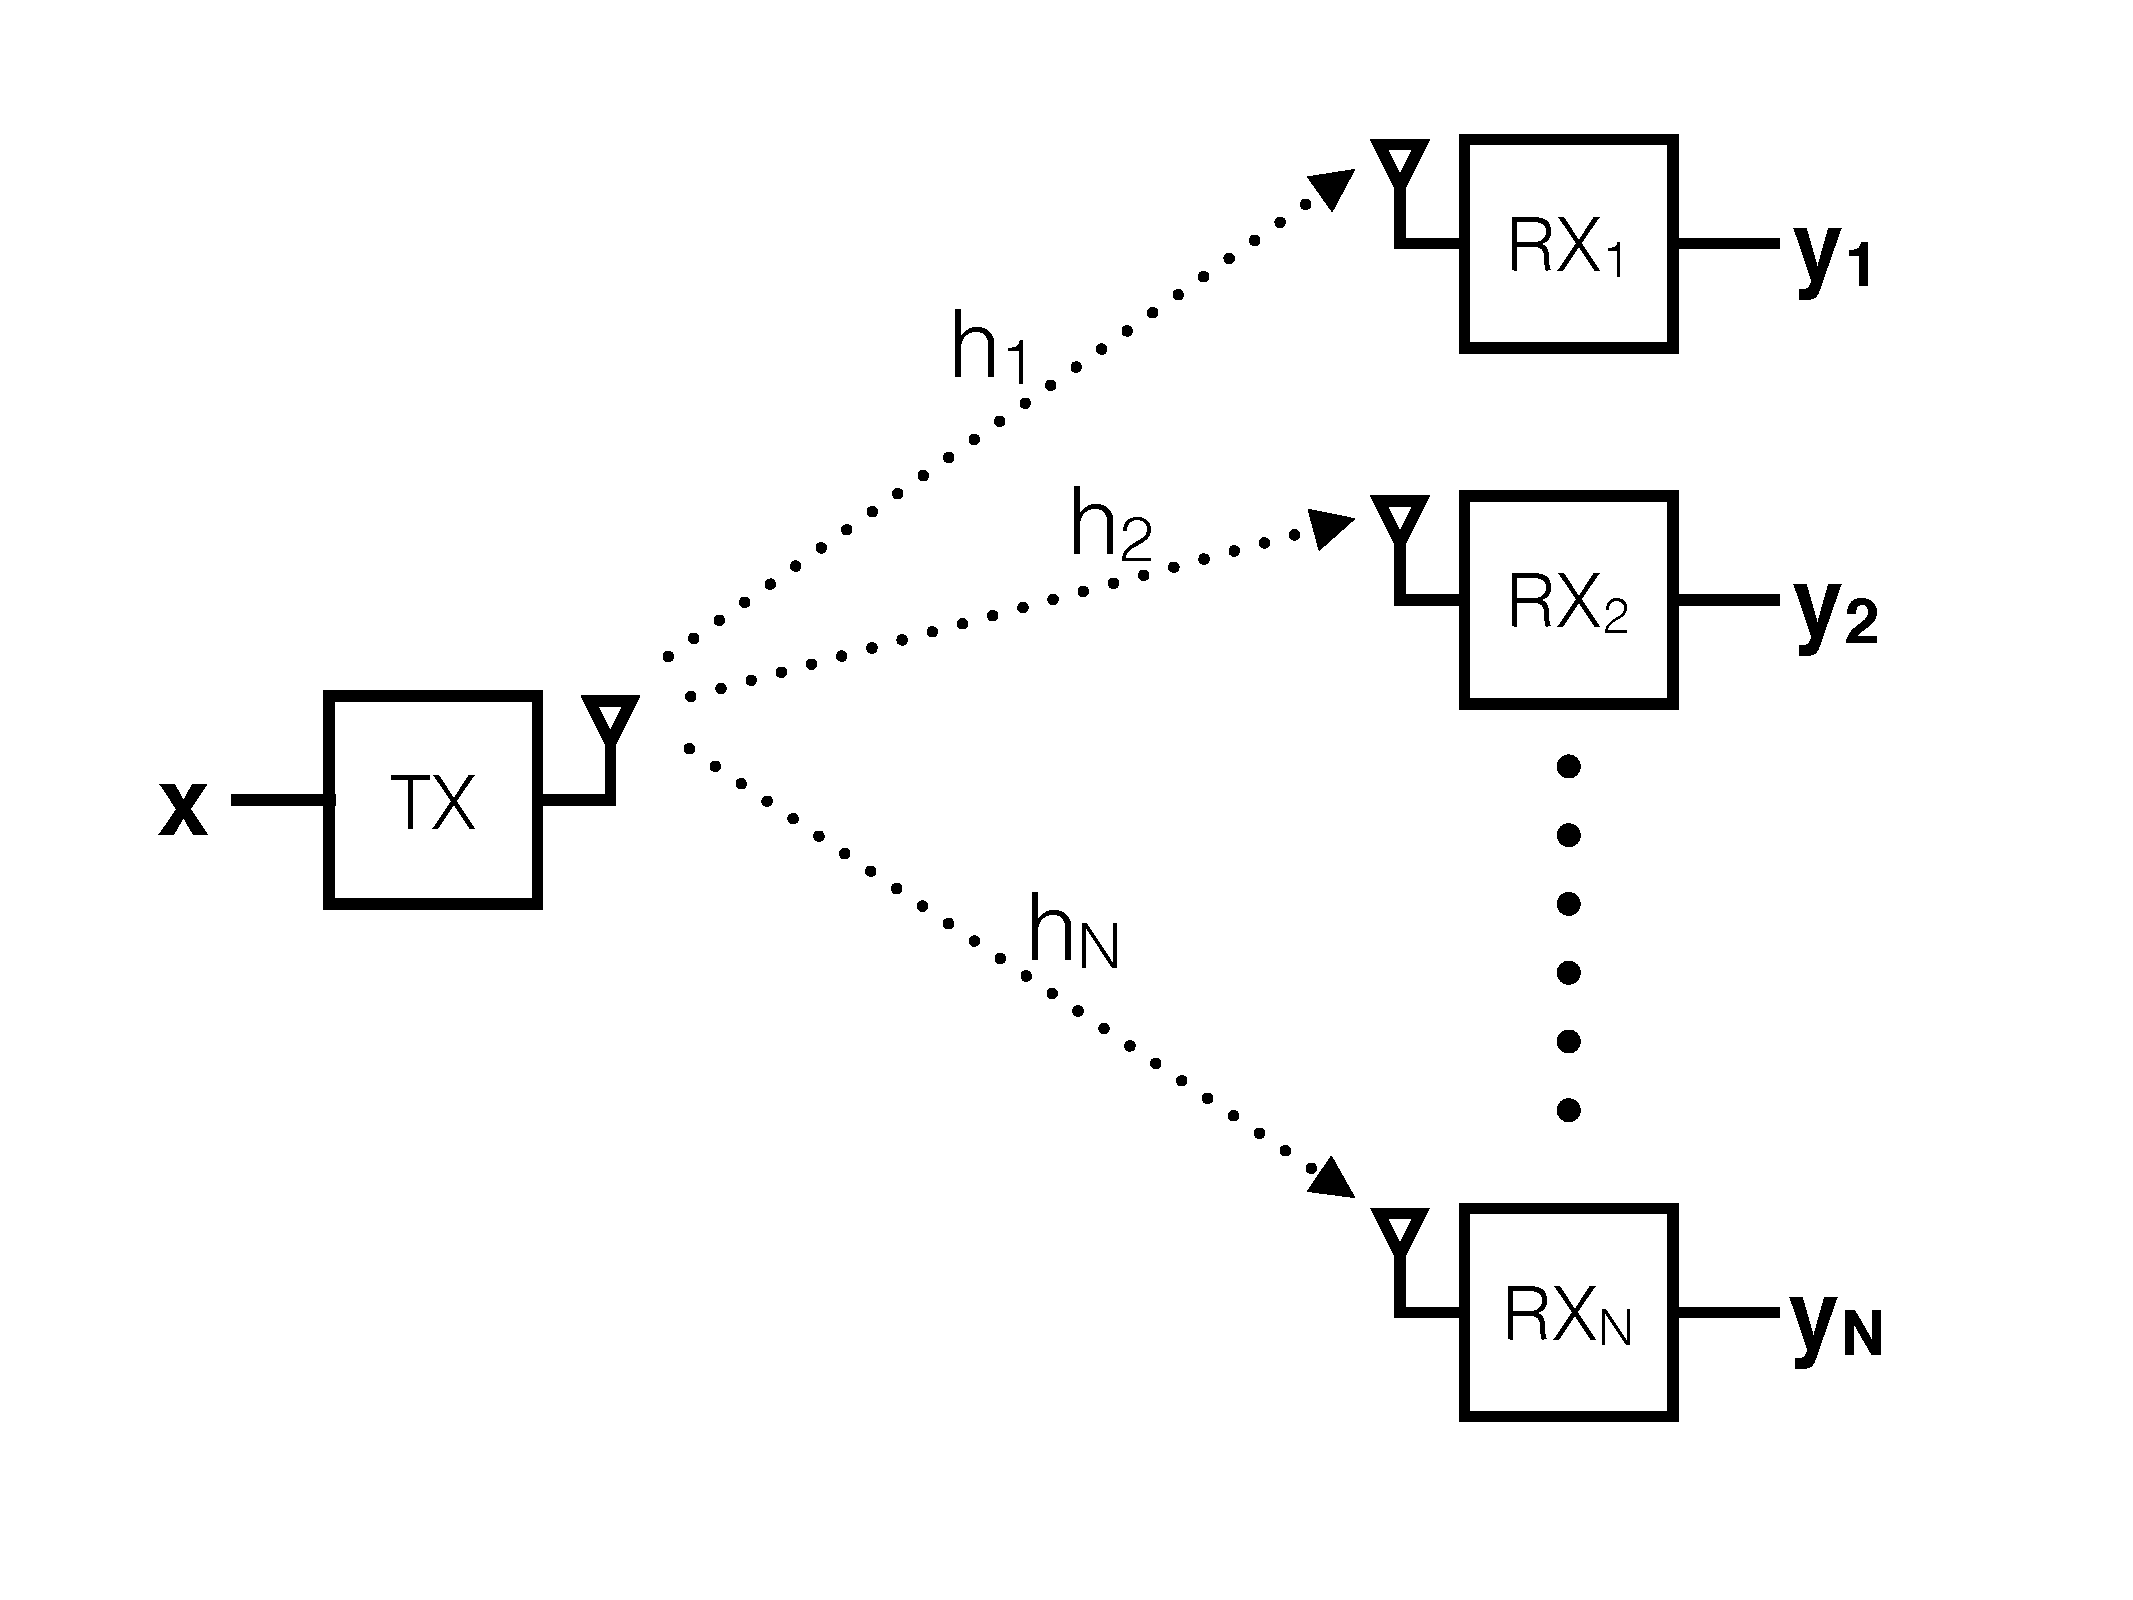
\includegraphics[width=0.45\textwidth]{figures/SIMO}
    \caption{A single-input multiple-output (SIMO) wireless system}
    \label{fig:simo}
\end{figure}

Let the transmitted signal be $x$ and each of the gateways receive a signal
$y_i$ through an AWGN channel that introduces independent noise $n_i$ at the
receivers. Since LoRa modulated signals are narrowband (up to 500 $kHz$) and
their symbol periods are large ($> 250~\mu s$) to remain
unaffected by inter-symbol interference, we get the following simplified
channel model.

\begin{align*}
y_i &= h_i x_i + n_i \\
\therefore h^*_i y_i &= h^*_i h_i x_i + h^*_i n_i \\
	&= \left| h_i \right|^2 x + n'_i
\end{align*}

Estimating the $h_i$ is only based on information available locally to the
receiver. The combined signals can then be coalesced by a joint decoder

\begin{align*}
y_{\text{combined}}
	&= \sum_{i=1}^N h^*_i y_i \\
	&= \sum_{i=1}^N \left| h_i \right|^2 x + \sum_{i=1}^N h^*_i n_i
\end{align*}

The first term is the combined signal while the second term is the combined
noise. However, the signals add up coherently while the noise, being
independent, adds up incoherently. This results in an overall increase in the
combined SNR which allows us to jointly decode a packet that would otherwise
not be decodable by any individula receiver.

\begin{align*}
SNR_{\text{combined}} &= \frac{\text{total signal power}}{\text{total noise power}} \\
	&= \frac{\left| \sum_{i=1}^N \left| h_i \right|^2 x \right|^2}{\sum_{i=1}^N \left| h^*_i n_i \right|^2} \\
	&\geq \frac{\left| \left| h_i \right|^2 x \right|^2}{\left| h^*_i n_i \right|^2} = SNR_i
\end{align*}

\subsection{LoRa Modulation}
\label{sec:lora}

{\color{blue}
Packet structure - extremely long preambles

Encoding as chirps

Spreading factors

How this enables power savings
}

\ac{LoRa}'s Physical layer is based on the \ac{CSS} modulation scheme and
integrates \ac{FEC} techniques. This makes it highly immune to interference,
resistant against multi-path fading and Doppler effects. Its unique features
allow for the reception of the signal even below the noise floor of the
receiver.
\ac{LoRa} modulation is both bandwidth and frequency scalable.
It can be easily adapted to work in narrow-band frequency hopping and wide-band direct sequence applications with only a few simple software configuration changes.
This modulation scheme enables low-power, long-range and high-efficiency operation.

\subsubsection{Spreading Factor (SF)}
\ac{LoRa}'s modulation design brings some additional features, \emph{e.g.} through the use of different \acp{SF}, multiple transmitted signals can occupy the same channel.
This is possible by encoding each transmission in a different chirp rate,
which LoRa denominates as \acp{SF}. Radio communications with different
\acp{SF} are orthogonal to each other and network separation using different
\acp{SF} is possible. This also permits coexistence with existing \ac{FSK}
based systems~\cite{Bor,LoRaWANSpec}.

In \ac{LoRa} modulation, the spreading of the spectrum is achieved by
generating a chirp signal that continuously varies in frequency. Each bit of
the message is embodied into multiple chips of information that are encoded as
up-chirps or down-chirps (\figref{upchirp}). Furthermore, \ac{SF} is defined
as the ratio between the symbol rate and the chip rate.%The number of chips user per symbol is determined by the formula in equation~\eqref{SFequation}.
For example, when using a \ac{SF} of 6 (SF6), 64 chips are used for every
symbol, correspondingly 128 and 4096 are used for SF7 and SF12. The use of
this modulation results in the capability of receiving signals with negative
\ac{SNR} of up to 19.5 dB below the noise floor. In comparison, most \ac{FSK}
systems need 8 to 10 dB above the noise floor in order to demodulate properly,
resulting in more than 27 dB difference in the link budget between the two
modulation systems, thus greatly increasing the range of a \ac{LoRa}
system~\cite{SX1276,SX1301}.

A higher \ac{SF} increases the \ac{SNR} and consequently the sensitivity and
range, but this also increases the transmission time of a message. Each level
of the \ac{SF} doubles the number of chips to be transmitted, thus increasing
the energy consumption and decreasing the data-rate in half. When using the
highest rate transmission, SF6, some special operations are required,
including the use of different headers for frame synchronization. Contrary to
some \ac{UNB} technologies, \ac{LoRa} does not require the use of an expensive
\ac{TCXO}, making the final cost of an end-device much lower~\cite{SX1276}.%Since spread spectrum takes advantage of a wider bandwidth, when \ac{LoRa} is used with large \acp{SF} and a \ac{UNB} (lower than 62.5kHz), the use of a more precise \ac{TCXO} crystal is strongly recommended in order to minimize the effect of frequency drift during operation.


% \subsubsection{Coding Rate (CR)}
% Coding Rate (CR) is the \ac{FEC} used by the LoRa modem that offers protection against bursts of interference.
% The sender adds redundancy in the messages by the use of \acp{ECC}.
% By default, \ac{LoRa} packet frames are encoded with the minimum CR of 4/5.
% A \ac{FEC} of 4/5 means that 4 useful bits are encoded into 5 transmission bits.
% As show in \tableref{FEC}, a higher CR offers more protection, but increases time on air.

\subsubsection{Frame Structure}
The \ac{LoRa} frame structure shown in \figref{frame} is composed of four main
fields. It starts with the preamble that is programmable from 6 to 65535
symbols, to which the radio adds and additional 4.25 symbols. The preamble is
followed by an optional frame header, which describes the length and \ac{FEC}
rate of the payload, and indicates the presence of an optional 16-bit CRC at
the end of the payload. The header is always transmitted with a 4/8 \ac{FEC}
rate, and has its own \ac{CRC} for increased protection of these fields. After
the optional header, there is the payload, which can contain 1 to 255 bytes
and the optional 16-bit \ac{CRC} at the end of the frame.

\begin{figure}
  \centering
  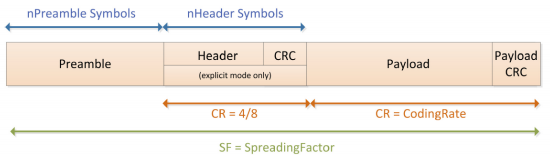
\includegraphics[width=\columnwidth]{figures/frame.png}
  \caption{LoRa PHY Frame Structure (with permission~\cite{SX1276})}
  \label{fig:frame}
\end{figure}

% \subsubsection{LoRa Gateway}
% The only gateway \ac{LoRa} chip currently on the market is the SemTech SX1301.
% It has two radios fronends with four programmable reception channels each.
% Each of the channels has a fixed channel bandwidth of 125 kHz and their frequency can be individually configured to use any of the two radios.
% For each channel, it is able to detect preambles corresponding to all data rates (SF7 to SF12) at all times.
% However, the gateway cannot demodulate more than eight packets simultaneously, because the SX1301 architecture separates the preamble detection from the data demodulation process (i.e the SX1301 only has eight demodulation blocks).
% Theoretically, it is possible to demodulate up to six transmissions per channel, one for each \ac{SF}, but SemTech has restricted the number of demodulation blocks.
% Therefore, the SX1301 was primarily designed to detect the preambles within a channel.
% SemTech states that personalized customer circuit designs with more than eight demodulation blocks can be made on request.

% The SX1301 has an separate \ac{GFSK} reception channel with adjustable bandwidth and bitrate, that can demodulate any legacy \ac{FSK} OR \ac{GFSK} signal.
% It also include an additional channel that is intended to be used as a high speed back-haul link to other gateways or infrastructure.
% It uses a fixed 125khz, 250khz or 500khz bandwidth and \ac{SF}, similar to the SX1276 chips found in client devices~\cite{SX1301}.

\subsubsection{Spectrum Regulation}
In different part of the world, the allocated bandwidth, frequency and local
regulations differ from each other. Even though LoRa operates using
unregulated spectrum, the increase in dwell time (Air-Time) rises the
probability of a collision in a contention based medium access. Thus, local
regulations may enforce duty-cycle or dwell time restrictions for certain
frequencies in order to implement fair use and avoid spectrum stagnation.

% The \ac{ETSI} has implemented such regulation on the European 868 MHz band that has 7 MHz of usable bandwidth.
% The regulations require the radio emitters to adopt duty-cycled transmission of 10\%, 1\% or 0.1\% depending on the sub-band.
% These transmissions also have a maximum transmit power as shown in table \tableref{DutyCycle}.
% In order to avoid duty-cycle limits, the transmitters need to implement two mechanisms: \ac{LBT} and \ac{AFA}.
% Both form a carrier sense mechanism that allow to sense the radio environment an only transmit on channels that are not yet occupied~\cite{ETSICompliance}.

The \ac{FCC}, which is the regulatory body in the \ac{US}, has no frequency
duty-cycle restrictions on the 915 MHz \ac{ISM} band that offers a total of 26
MHz of bandwidth. Instead, they require each radio emitter to adopt a
\ac{FHSS} scheme. Channel hopping should be employed in a pseudo-random nature
across at least 25 or 50 channels in order to be able to transmit at a peak
power output of +24 dBm (250 mW) and 30 dBm (1 W) respectively. Each
transmission should not exceed a dwell time of 400 milliseconds within a
period of 20 seconds~\cite{FCC15, FCCCompliance}. The maximum dwell time makes
the lowest \ac{LoRa} data-rates (\ac{SF} 11 and 12) not usable, as
transmitting the preamble alone already takes longer than 400 milliseconds.

\subsection{LoRaWAN}
\label{sec:lorawan}

The LoRa Wide-Area Networking (LoRaWAN) protocol works on top of the LoRa
modulation layer to create an LP-WAN network capable of bi-directional data
transfer. Its functionality is analogous to the Networking and transport
layers (layers three and four) in the typical OSI design. LoRaWAN networks
are designed to be simple star-topologies that have client devices directly
communicating with a gateway that is connected to the internet over ethernet
or cellular links. LoRaWAN defines three main device classes: bi-directional
end-devices with downlink followed by uplink (Class A), bi-directional
end-devices with transmission slots scheduled for downlink (Class B) and
always-on bi-directional devices (Class C). Class A is primarily intended for
sensors, Class B is intended for sensors with actuators while Class C is
intended for powered devices that require low-latency. Gateways are very
simple and relatively inexpensive forwarders that send received packets to a
cloud LoRaWAN server and can be commanded by the server to transmit data to
clients at a specific time. Packet decoding, managing acknowledgements and
MAC parameters like data-rate and power-level are decided at a LoRaWAN
server. The LoRa community often refers to the system as having a
``MAC-in-the-Cloud" design.

LoRaWAN allows and encourages its users to deploy their own gateways. In this
paper, we refer to these as user-deployed gateways (UGW). These UGWs are
completely unplanned and on low-bandwidth, unreliable internet connections
(compared to cellular base-stations which are extensively planned and have
dedicated optic fiber connections). In pilot deployments, we've observed the
same transmission being received by multiple gateways. In this paper, we
leverage this observation combined with the diversity from unplanned UGW
deployments to extend the coverage of higher data-rates in our network.
Low-power devices which can now transmit at higher data rates thus end up
saving energy to shorter transmit time.

{\color{blue}

Q. how do we save client power while sticking to LoRaWAN?
}